% ---------------------------------------------------- %
%                CONFIGURATION                         %
% ---------------------------------------------------- %

\documentclass[twoside]{article}

\usepackage{lipsum} % Package to generate dummy text throughout this template
\usepackage{amsmath}
\usepackage[sc]{mathpazo} % Use the Palatino font
\usepackage[T1]{fontenc} % Use 8-bit encoding that has 256 glyphs
\linespread{1.05} % Line spacing - Palatino needs more space between lines
\usepackage{microtype} % Slightly tweak font spacing for aesthetics
\usepackage[hmarginratio=1:1,top=32mm,columnsep=20pt,left=0.8in,right=0.8in]{geometry} % Document margins
\usepackage{multicol} % Used for the two-column layout of the document
\usepackage[hang, small,labelfont=bf,up,textfont=it,up]{caption} % Custom captions under/above floats in tables or figures
\usepackage{booktabs} % Horizontal rules in tables
\usepackage{float} % Required for tables and figures in the multi-column environment - they need to be placed in specific locations with the [H] (e.g. \begin{table}[H])
\usepackage{hyperref} % For hyperlinks in the PDF

\usepackage{lettrine} % The lettrine is the first enlarged letter at the beginning of the text
\usepackage{paralist} % Used for the compactitem environment which makes bullet points with less space between them

\usepackage{abstract} % Allows abstract customization
\renewcommand{\abstractnamefont}{\normalfont\bfseries} % Set the "Abstract" text to bold
\renewcommand{\abstracttextfont}{\normalfont\small\itshape} % Set the abstract itself to small italic text

\usepackage{titlesec} % Allows customization of titles
\renewcommand\thesection{\Roman{section}} % Roman numerals for the sections
\renewcommand\thesubsection{\Roman{subsection}} % Roman numerals for subsections
\titleformat{\section}[block]{\large\scshape\centering}{\thesection.}{1em}{} % Change the look of the section titles
\titleformat{\subsection}[block]{\large}{\thesubsection.}{1em}{} % Change the look of the section titles

\usepackage{fancyhdr} % Headers and footers
\pagestyle{fancy} % All pages have headers and footers
\fancyhead{} % Blank out the default header
\fancyfoot{} % Blank out the default footer
\fancyhead[C]{Efficient Coding Hypothesis and an Introduction to Information Theory $\star$ September 2014} % Custom header text
\fancyfoot[RO,LE]{\thepage} % Custom footer text

\usepackage{graphicx}


% ---------------------------------------------------- %
%                CONFIGURATION                         %
% ---------------------------------------------------- %



% ---------------------------------------------------- %
%                   	TITLE                          %
% ---------------------------------------------------- %

\title{\vspace{-15mm}\fontsize{24pt}{10pt}\selectfont\textbf{Efficient Coding Hypothesis and an Introduction to Information Theory}} % Article title
\author{Lay Kuan Loh \& Mihovil Bartulovic}
\date{\today}

% ---------------------------------------------------- %
%                   	TITLE                          %
% ---------------------------------------------------- %



\begin{document}

\maketitle % Insert title

\thispagestyle{fancy} % All pages have headers and footers




% ---------------------------------------------------- %
%                   	ABSTRACT                       %
% ---------------------------------------------------- %

\begin{abstract}

\noindent The Efficient Coding Hypothesis, proposed by Barlow 1961, suggests that sensory relays recode sensory messages, so that their redundancy is reduced, but little information is lost. Coding to reduce redundancy not just eliminates wasteful neural activity, but also organizes sensory information such than an internal model of the environment causing the past sensory inputs to built up, while the current sensory situation is represented in a way that simplified the task of the part of the nervous system which is responsible for learning and conditioning. Studies on neurons using this hypothesis have shown promising evidence of its validity when applied to neurons. We also discuss some criticism of the hypothesis' use and their merits.

\end{abstract}

% ---------------------------------------------------- %
%                   	ABSTRACT                       %
% ---------------------------------------------------- %








% ---------------------------------------------------- %
%                   	INTRODUCTION                   %
% ---------------------------------------------------- %

\begin{multicols}{2} % Two-column layout throughout the main article text

\section{Introduction}

\lettrine[nindent=0em,lines=3]{I}nformation Theory represents the necessary basis of the modern information and communication technologies. Without it, many of today's technologies would be unavailable.

Bits are the standard choice of unit in Information Theory. The core theorems of Information Theory set measures for the quantity of information, upper bound for loss-less compression of information, and for the highest speed for the information to be transferred trough a channel with or without noise. 

Although Information Theory does not give practical solutions for upper bounds that it sets, the theory behind it is a vital step to practical implementation. The transfer of information should be fast, precise, energy efficient and it should work regardless the inevitable interference and noises in the channel. Information Theory presents the necessary basis for efficiently coding and compressing various types of information such as text, images, and sound. 

The Efficient Coding Hypothesis is one of the quantitative links between the statistical and structural properties our visible surroundings. It is a core theory in Information Theory and has inspired new directions in neuroscience. This hypothesis suggests that a group of neurons should encode information as compactly as possible in order to maximize efficient utilization of resources, meaning that the information carried by one neuron should not be redundant to the information which is carried by the other neurons. 

\begin{figure}[H]
	\caption{
		Model of how visual information is transmitted from the surroundings to the brain.
	}
	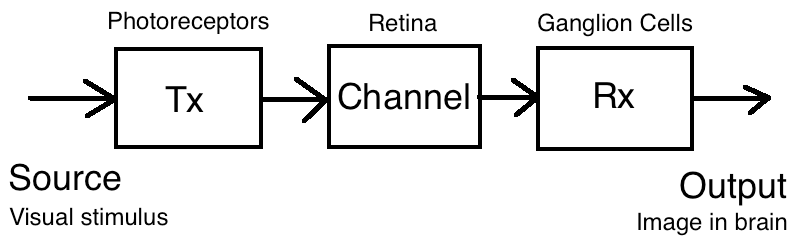
\includegraphics[width=0.5\textwidth]{model}
	\label{fig:model}
\end{figure}

Testing the Efficient Coding Hypothesis is impractical as estimating information-theoretic quantities requires large amounts of data, and common estimators of information are heavily biased. Therefore, it is hard to achieve a good estimation from any set of given data. Nonetheless, successful experimental results have been achieved, which will be described in this paper. Some criticisms of the application of this theory are also described, along with a discussion of their merits. 

% ---------------------------------------------------- %
%                   	INTRODUCTION                   %
% ---------------------------------------------------- %



% ---------------------------------------------------- %
%                      BARLOW 1961                     %
% ---------------------------------------------------- %

\section{Possible Principles Underlying the Transformations of Sensory Messages}

Barlow 1961 discusses three hypotheses about sensory relays:
\begin{itemize}
	\item Hypothesis 1: Sensory relays detect certain "passwords" in incoming messages that have a particular key significance.
	\item Hypothesis 2: Sensory relays are filters whose "pass characteristics" can be controlled in accordance with the requirements of the other part of the nervous system.
	\item Hypothesis 3: Sensory relays recode sensory messages, extracting signals of high relative entropy from the highly redundant sensory input.
\end{itemize}
His paper is not a discussion of the physiological mechanisms of sensory pathways, but an attempt to formulate ideas about operations which these mechanisms do. The idea behind all of the three above mentioned hypothesis comes from experimental results, not merely from abstract speculations on this topic. 

In Hypothesis 1, specific classes of stimuli act as "releasers" and evoke specific responses. These classes of stimuli are thought of as "passwords" which have to be distinguished from other stimuli and it is suggested that their detection may be the important function of sensory relays. For instance, a frog's visual system has a limited range of visual responses. A moving object elicits a sequence of reactions, such as the frog going into alert, or hopping forward and snapping at it. This hypothesis says that since animals respond differently to specific stimuli, their sensory pathways must have mechanisms for detecting such stimuli and discriminating between them. 

In Hypothesis 2, sensitivity of one type of stimulus might be increased while another is decreased. Combined with Hypothesis 1, this means the whole characteristic of relay could change, so that, in effect, the "password" is altered. Thus, relays act as control points at which the flow of information is modulated according to the requirements of the other parts of the nervous system.

Hypothesis 1 argued about existence of preset mechanisms for detecting and passing on restricted classes of key signals. Hypothesis 2 postulated that the acceptance or rejection of messages might be controlled from somewhere else - either be a temporary change or a permanent adjustment for the sensory relays. The remaining question is: is the current input new information? If not, it should be marked as redundant and rejected. 

Several assumptions need to be made for Hypothesis 3:
\begin{itemize}
	\item Sensory pathways are noiseless and use discrete time signals.
	\item The discrete time signals for any one fiber and time interval are binary impulses which are either present or absent.
	\item The capacity of a nerve pathway is constrained as such: number of fibers $F$ is constant, number of discrete time intervals per second $R$ is also constant, and the average number of impulses per second in one fiber $I$ is variable.
\end{itemize}

These assumptions are not justified by experimental results, but are mentioned due to potential generality of the problem. FitzHugh 1957 criticized these assumptions where an evidence is produced which tells us that it is not important if a single impulse in the short time interval is there or not but the cumulative number of impulses in a longer time interval is the one who carries the information. 

Hypothesis 3 states that sensory relays recode sensory messages so that their redundancy is reduced, but little information is lost. A "message" it is assumed to be a set of signals, i.e. a particular pattern of impulses along a set of $N$ fibers during the time interval $T$. Denoting $\mathbb{P}_m$ as the probability of the message $m$ in such an ensemble, the information attributed to $m$ is $H_{m}=-\log \mathbb{P}_m$. The average information of all of the messages is thus the summation of information of all members of the ensemble.

\begin{align} \label{eq:1}
	H_{av}= \sum_m \mathbb{P}_m \log \mathbb{P}_m
\end{align}

The rate of flow of information is $\dfrac{H_{av}}{T}$, where $T$ is the average duration of messages from the ensemble.

\begin{align} \label{eq:2}
	T = \sum_m \mathbb{P}_m \mathbb{T}_m.
\end{align}

The capacity $C$ of a channel is equal to the greatest rate of flow of information that can be passed down it. The capacity of a nerve pathway is

\begin{align} \label{eq:3}
	C = - FR \left[\frac{I}{R} \log \frac{I}{R} +\left(1-\frac{I}{R} \right) \log  \left(1-\frac{I}{R} \right) \right].
\end{align}

The relative entropy of the messages is $\dfrac{H}{CT}$, and thus making the redundancy $1-\dfrac{H}{CT}$. The channel capacity is maximum if $I = \dfrac{R}2$. In normal circumstances $I < \dfrac{R}{2}$, thus a decrease in redundancy of the sensory relay can only be done by decreasing the average frequency of impulses being used to transfer a message. Therefore, for a given class of input messages, relays will choose the code that requires the smallest average expenditure of impulses in the output signal. Hence, reduction of redundancy is an important principle guiding the organization of sensory messages and it is carried out at relays in the sensory pathways.

The main difference between the last hypothesis and the first two is that the first two consist of possible principles for selecting some sensory messages while rejecting others. The selected messages are considered to be infrequent, and all of the rejected messages would be classified in the same way, thus disregarding a large part of the data. Hypothesis 3, however, preserves the given information.

In the next section, we present a paper by Simoncelli 2003 on critiques of the efficient coding hypothesis. 






% ---------------------------------------------------- %
%                     SIMONCELLI 2003                  %
% ---------------------------------------------------- %

\section{Vision and the Statistics of the Visual Environment}

In his paper Simoncelli has several criticisms about articles relating to the Efficient Coding Hypothesis that were published in the last several years. He argues some misconceptions about the theory behind Efficient Coding Hypothesis, and also criticizes some experimental results.

\subsection{Criticisms of hypothesis}

\noindent\textbf{The purpose of Vision}

Firstly, Simoncelli suggests that the efficient coding of visual information is not important, as the purpose of vision is not to encode and reconstruct the visual world. The hypothesis does not take into account how the information that has been extracted is to be used, which could be an advantage as one does not need to specify what is being represented, or a limitation as goals are relevant for visual processing. There are other, more complete theories such as Bayesian estimation which take the statistical structure of the environment and goal into account.

\noindent\textbf{Relevance of Information Theory}

The Efficient Coding Hypothesis is not important because brain does not work with bits as an unit of information. 

This is not completely valid, as whatever unit of information the brain works with could likely be represented with bits using a suitable mapping, so the definition of information is relevant to the brain as bits are a universal currency of information.

However, this criticism is partly relevant as some information the brain holds are more important than others. Also, the brain does not perfectly reconstruct everything it sees. Evidence for this is the filling-in phenomena, which completes missing information at the blind spot of the eye. Also, objects at the periphery of one's vision cannot be seens as clearly as objects in one's direct line of sight. In a "Selective Attention Test" by Chabris et. al. 2011, study participants were asked to watch a short video in which six people, three in white shirts and three in black shirts pass basketballs around. While they watched, they were to concentrate on the people in white shirts. At some point, a person wearing a  gorilla suit strolled into the middle of the action and spent 9 seconds on camera. Half of the did not notice the gorilla as there were not focused on it. Studies on blind people show that their visual cortices degrade after a while, while their auditory physiology develops to make them more sensitive to sound to compensate. Other animals are also selective in the visual signals they are alert to. For instance, one is advised to which is why one is advised to keep still upon meeting a cobra, as they cannot see stationary objects well. 

\noindent\textbf{Evolution may not lead to the globally optimal efficient coding solution}

The efficient coding hypothesis may lead to the best possible solution for efficient coding of information, but evolution would not necessary find this solution, as the brain does not drastically change between generations. The coding solution it does use could be a locally optimal one, but not the global optimum, as there is a limit to how much evolutionary forces can change a structure that is already set in place. 

\noindent\textbf{Experimental Observed Dependency}

Some experimental data from multi-neuron recordings show correlation, synchronization, or other forms of statistical dependency between neurons. However, most of these data came from experiments that did not use naturalistic stimuli. Also, other studies suggest that responses to natural stimuli in the primary visual cortex (V1) are relatively independent. 

\noindent\textbf{Over-representation in cortex}

Critics argue that the number of neurons devoted to processing sensory information seems to expand as one goes deeper into the system, suggesting that the brain increases redundancy. However, this argument assumes incorrectly. that the coding capacity of all neurons is the same. 

\noindent\textbf{Definition of input and output}

The Efficient Coding Hypothesis depends on the assumptions about the probability distribution of natural images and the definition of the neural response, both of which are unconstrained. When applying the hypothesis, one must be careful about the definitions used in order to satisfy it. For instance, the input distribution is assumed to be well represented by a collection of calibrated 'naturalistic' images. The type of neurons used must also be clearly stated.

\subsection{Testing the Hypothesis}

Although the Efficient Coding Hypothesis is already 50 years old, it is only now being more widely explored today, due to better information on neural signal processing, and better mathematical and engineering tools to process large amounts of experimental data.

The two basic approaches for testing the Efficient Coding Hypothesis are to focus on examining statistical properties of neural responses under natural stimuli, or using statistical properties of natural images to constrain and derive a model for the early sensory processing.

In the following sections, we present in-depth discussions of two such studies which support the hypothesis. 

% ---------------------------------------------------- %
%                     SIMONCELLI 2003                  %
% ---------------------------------------------------- %




% ---------------------------------------------------- %
%                	NIRENBERG 2001                     %
% ---------------------------------------------------- %

\section{Retinal ganglion cells act largely as independent encoders}

Correlated firing among neurons is widespread in the visual system, but its importance for encoding visual information is unclear. To study this, Nirenberg et. al., 2001 presented the retina with natural stimuli and computed the responses of the output cells, the ganglion cells. They used information theoretic techniques to measure the amount of information about the stimuli that can be obtained from the cells under correlated firing and non-correlated firing. They found that more than 90\% of the information about the stimuli can be obtained from the cells with uncorrelated firing, suggesting that ganglion cells act largely independently to encode information, simplifying the problem of decoding their activity. 

To perform the study, Nirenberg et. al., 2001 stimulated pairs of isolated mouse retina using natural movies. The stimuli were each 7 seconds long and repeated 300 times, and the ganglion cell responses were recorded. Data used had to be clean of contaminating spikes from other cells, and that both responses had to have average firing rates. 

To find the degree of correlated activity for each pair, the excess correlated fraction (ECF) was found. ECF is the fraction of correlated spikes produced by the pair above chance, taking into account correlations induced by the stimulus. The ECFs ranged from -1\% to 34\%. 

To measure the amount of information the pairs of ganglion cells carried about the stimuli when their correlations were taken into account, information theoretic techniques were used. Each movie was treated as a series of segments of fixed temporal length, with each segment regarded as a separate stimulus. The movie was presented several hundred times to generate a large set of responses (spike trains) to each segment. This allowed the authors to estimate the probability of getting a particular pair of responses given a particular movie segment - that is, to estimate $\mathbb{P}(r_1,r_2|s)$, where $r_1$ was the response of cell 1, $r_2$ was the response of cell 2 and $s$ was the movie segment. Given these conditional probabilities, the amount of information $I$ between the responses and the stimulus segments was found using the expression:


\begin{align}\label{eq:info-theory}
	I 
		&= -\sum_{r_1,r_2}\mathbb{P}(r_1,r_2)\log_2\mathbb{P}(r_1,r_2) \\
  		&+ \sum_s\mathbb{P}(s) \sum_{r_1,r_2}\mathbb{P}(r_1,r_2|s)\log_2\mathbb{P}(r_1,r_2|s)
\end{align}


where $\mathbb{P}(r_1,r_2)$ is found by taking $\mathbb{P}(r_1,r_2) = \sum_s \mathbb{P}(r_1,r_2|s)\mathbb{P}(s)$, and $\mathbb{P}(s)$ is the probability that a given stimulus segment $s$ occurred. 

To examine how important correlation is in encoding visual information, the amount of information that would be lost if the correlations in the responses of the pair of ganglion cells were ignored was examined. To ignore the correlations, the conditional probability distributions of the two responses, $\mathbb{P}(r_1,r_2|s)$, as the product of their individual probability distributions, $\mathbb{P}(r_1|s)$ and $\mathbb{P}(r_2|s)$. $\mathbb{P}(r_1|s)\mathbb{P}(r_1|s)$ to estimate the probability of a stimulus given a response. As $\mathbb{P}(r_1|s)\mathbb{P}(r_1|s)$ is not quite the true distribution, using it should lead to a loss of information. 

Therefore, the amount of independent information is given by

\begin{align}
	I_{IND} 
		&= -\sum_{r_1,r_2}\mathbb{P}(r_1,r_2|s)\log_2\mathbb{P}(r_1|s)\mathbb{P}(r_2|s) \\
		&+ \sum_s\mathbb{P}(s) \sum_{r_1,r_2}\mathbb{P}(r_1,r_2|s)\log_2\mathbb{P}(r_1|s)\mathbb{P}(r_2|s) 
\end{align}

The amount of information in bits lost, $\Delta I$, is given by 
\begin{align}
	\Delta I 
		&= I - I_{IND} \\
		&= \sum_s\mathbb{P}(s) \sum_{r_1,r_2}\mathbb{P}(r_1,r_2|s) \log_2 \frac{\mathbb{P}(r_1,r_2|s)}{\mathbb{P}(r_1|s)\mathbb{P}(r_2|s)} \\
		&- \sum_{r_1,r_2}\mathbb{P}(r_1,r_2) \log_2 \frac{\mathbb{P}(r_1,r_2)}{\sum_s \mathbb{P}(r_1|s)\mathbb{P}(r_2|s) \mathbb{P}(s)} 
\end{align}

$\Delta I$ is very small, as most pairs lost less than 10\% of information. If there were pairs of ganglion cells with higher degrees of correlation than the maximum 34\% observed, more information loss could have occurred. This finding means that strategies used to decode ganglion cell activity, which treat the cells as independent encoders are reasonable, as they can capture more than 90\% of the information the cells carry. Furthermore, the activity of any given ganglion cell can be evaluated separately from other cells, without accounting for other cells in the population. This allows the problem of decoding population activity to be significantly simplified, as much less data is needed to analyze the uncorrelated case as opposed to the correlated case. 

Several concerns with the study are that capturing more than 90\% in ganglion cell activity may not be enough to fully understand its activity. Also, perhaps correlation should not be ignored for the activity of a larger population of cells than just pairs of cells studied here. 

% ---------------------------------------------------- %
%                	NIRENBERG 2001                     %
% ---------------------------------------------------- %






% ---------------------------------------------------- %
%                    LAUGHLIN 1981                     %
% ---------------------------------------------------- %

\section{A Simple Coding Procedure Enhances a Neuron's Information Capacity}

This study by Laughlin 1981 validates Barlow 1961's suggestion that redundancy reduction is an important principle in neural coding. Laughlin that the receptors of large monopolar cells (LMCs), the first order interneurons of the insect compound eye, have a compressive intensity-response function corresponding to the background intensity. Instead of absolute intensity, the LMC's contrast-response function matches the range of contrasts encountered in natural scenes, which increases the efficiency.

A neuron has a limited range of responses that can represent the states of its inputs. If its sensitivities are too high, inputs would saturate the response, and input outside the response range would be lost. If sensitivities are too low, the response range would correspond to very large ranges of input, and many parts of it would therefore be underutilized. Information theory suggests that the most efficient way to apportion the neuron's limited response range is to maximize entropy by encoding inputs so that all response levels are used with equal frequency. 

In the simplest case, shown in Figure~\ref{fig:laughlin1981-fig1}, a neuron represents a single input parameter with a single output parameter. Maximum entropy is achieved when inputs are amplified in proportion to their expected frequency of occurrence. Larger portions of the response range are used for better resolution of common events, and smaller portions for improbable events. 

\begin{figure}[H]
	\caption{
		\textsc{Upper diagram:} Probability density function for stimulus intensities. \\ \textsc{Lower diagram:} Intensity-response function that implements the strategy. \\ Maxmimizing a neuron's information capacity by ensuring that all response levels are used with equal frequency. Intervals between each response level encompasses an equal area under the intensity distribution, so each state is used with equal frequency.
	}
	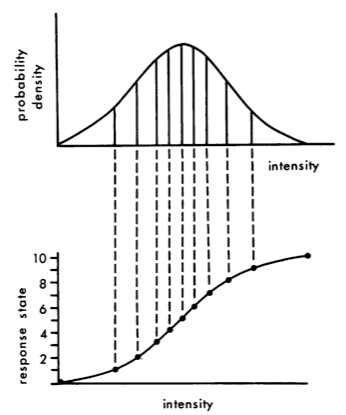
\includegraphics[width=0.45\textwidth]{laughlin1981-fig1}
	\label{fig:laughlin1981-fig1}
\end{figure}

To test this hypothesis, Laughlin compared contrast-response functions with contrast levels measured in natural scenes, such as lakeside vegetation in LMCs. Relative intensities were measured across the scenes with a detector with spectral sensitivity similar to a fly monopolar cell. Contrast values were obtained by dividing each scan into intervals. Within each interval, the intensity $\bar{I}$ was found, and for each data point the fluctuation about the mean $\delta I = I - \bar{I}$ was computed. Finally, the contrast $\displaystyle\frac{\Delta I}{\bar{I}}$ was found. The contrast-response function approximates the form of the cumulative distribution function for contrast levels in natural scenes~\ref{fig:laughlin1981-fig2}, indicating that the neurons uses the strategy for efficient coding suggested by information theory. Therefore, as expected, there is little redundancy associated with the LMC response to natural scenes. 

\begin{figure}[H]
	\caption{
		The contrast-response function of light adapted fly LMCs compared to the cumulative probability function for natural contrasts ($50^\circ$ interval).
	}
	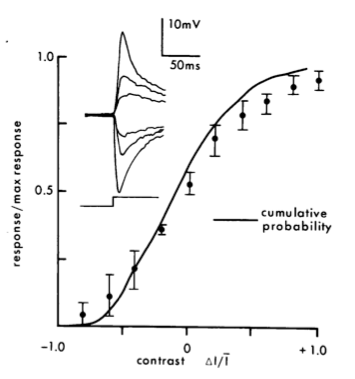
\includegraphics[width=0.45\textwidth]{laughlin1981-fig2}
	\label{fig:laughlin1981-fig2}
\end{figure}

While this study shows promising evidence for the Efficient Coding Hypothesis, it would be good to see similar results from testing neurons from other types of organisms, as well as examining the difference in efficiency achieved by natural stimuli as compared to the efficiency achieved with man-made stimuli.

% ---------------------------------------------------- %
%                    LAUGHLIN 1981                     %
% ---------------------------------------------------- %




% ---------------------------------------------------- %
%                      CONCLUSIONS                     %
% ---------------------------------------------------- %

\section{Conclusions}

Recent interest in Efficient Coding Hypothesis has led to interesting theoretical and experimental results. They suggest that neural system reduce redundancy by extracting signals of high relative entropy. For instance, Laughlin 1981 showed that the entropy of a neuron’s limited response range is maximized by encoding inputs so that all response levels are used with equal frequency. Thus, natural stimuli optimize the neuron's response. Several critiques of the applications of the Efficient Coding Hypothesis suggest it is improbable that the Efficient Coding Hypothesis is the the only principle behind sensory system design. However, experimental results show it clear that it plays an important role.

% ---------------------------------------------------- %
%                      CONCLUSIONS                     %
% ---------------------------------------------------- %


% ---------------------------------------------------- %
%                 	REFERENCE LIST                     %
% ---------------------------------------------------- %

\begin{thebibliography}{99} 

\bibitem[Barlow 1961]{Barlow:1961dg}
Barlow, H.~B. (1961).
\newblock Possible Principles Underlying the Transformations of Sensory Messages.
\newblock {\em Sensory communication}, (1961):217-234.

\bibitem[Laughlin, 1981]{Laughlin:1981dg}
Laughlin, S. (1981).
\newblock A Simple Coding Procedure Enhances a Neuron's Information Capacity.
\newblock {\em Z. Naturforsch}, 36.910-912 (1981): 51.

\bibitem[Nirenberg et. al., 2001]{Nirenberg:2001dg}
Nirenberg, S., Carcieri, S.~M., Jacobs, A.~L., \& Latham, P.~E. (2001).
\newblock Retinal ganglion cells act largely as independent encoders.
\newblock {\em Nature}, 411(6838), 698-701.

\bibitem[Simoncelli 2003]{Simoncelli:2003dg}
Simoncelli, E.~P. (2003).
\newblock  Vision and the statistics of the visual environment.
\newblock {\em Current opinion in neurobiology}, 13(2), 144-149.

\bibitem[Meister et. al., 1995]
Meister M., Lagnado L., Baylor D.~A. (1995). 
\newblock Concerted signaling by retinal ganglion cells. 
\newblock {\em Science 1995}, 270:1207-1210.

\bibitem[Vinje 2000]
Vinje W.~E., Gallant J.~L. (2000).
\newblock Sparse coding and decorrelation in primary visual cortex during natural vision
\newblock {\em Science 2000}, 287:1273-1276.

\bibitem[Chabris et. al. 2011]
Chabris C.~F., Daniel J.~S. (2011).
\newblock The invisible gorilla: And other ways our intuitions deceive us. \newblock {\em Random House LLC}, 2011.

 
\end{thebibliography}

% ---------------------------------------------------- %
%                 	REFERENCE LIST                     %
% ---------------------------------------------------- %


\end{multicols}

\end{document}


% ---------------------------------------------------- %
